\documentclass{config}
\usepackage{lipsum}
\usepackage{graphicx}
\usepackage{setspace}
\usepackage{amssymb}
\usepackage{listings}
\usepackage{appendix}
\usepackage{hyperref}




\newcommand{\lesss}{\rotatebox[origin=c]{90}{$\land$}}
\newcommand{\less}{\ \lesss\ }

\newcommand{\biggg}{\rotatebox[origin=c]{90}{$\lor$}}
\newcommand{\bg}{\ \biggg\ }

\lstdefinestyle{customc}{
  belowcaptionskip=1\baselineskip,
  breaklines=true,
  frame=L,
  xleftmargin=\parindent,
  language=C,
  showstringspaces=false,
  basicstyle=\footnotesize\ttfamily,
  keywordstyle=\bfseries\color{green!40!black},
  commentstyle=\itshape\color{purple!40!black},
  identifierstyle=\color{blue},
  stringstyle=\color{orange},
}

\lstdefinestyle{customasm}{
  belowcaptionskip=1\baselineskip,
  frame=L,
  xleftmargin=\parindent,
  language=[x86masm]Assembler,
  basicstyle=\footnotesize\ttfamily,
  commentstyle=\itshape\color{purple!40!black},
}

\lstset{escapechar=@,style=customc}


\title{Rapport ECL - Template} %Titre du fichier

\begin{document}
\lstset{language=[x86masm]Assembler} 
\begin{spacing}{1.2}
%----------- Informations du rapport ---------

\titre{Bureau d'Etude en Mécanique \\ Relais d'accessoires} %Titre du fichier .pdf

\enseignant{M. Hugues \textsc{Templier}}%Nom des élèves

\eleves{Jérôme \textsc{Plé} \\
		Alexandre \textsc{Ratieuville-Ogier}}%Nom des élèves

%----------- Initialisation -------------------
        
\fairemarges %Afficher les marges
\fairepagedegarde %Créer la page de garde
\tabledematieres %Créer la table de matières


%------------ Corps du rapport ----------------



%\begin{center}
%\includegraphics[scale=0.6]{carte_sabre_lite_image2.jpg}
%\captionof{figure}{Vu sur System Viewer de notre programme fonctionnant sur la carte SabreLite}
%\end{center}

\newpage
\section{Introduction}

Dans notre phase d'apprentissage des différentes notions en mécanique, nous avons comme objectif de concevoir un relais d'accessoires pour un réacteur d'avion.
Ce relais est un élément clef pour le réacteur. En effet, il permet notamment de démarrer le réacteur d'un avion.



\begin{center}
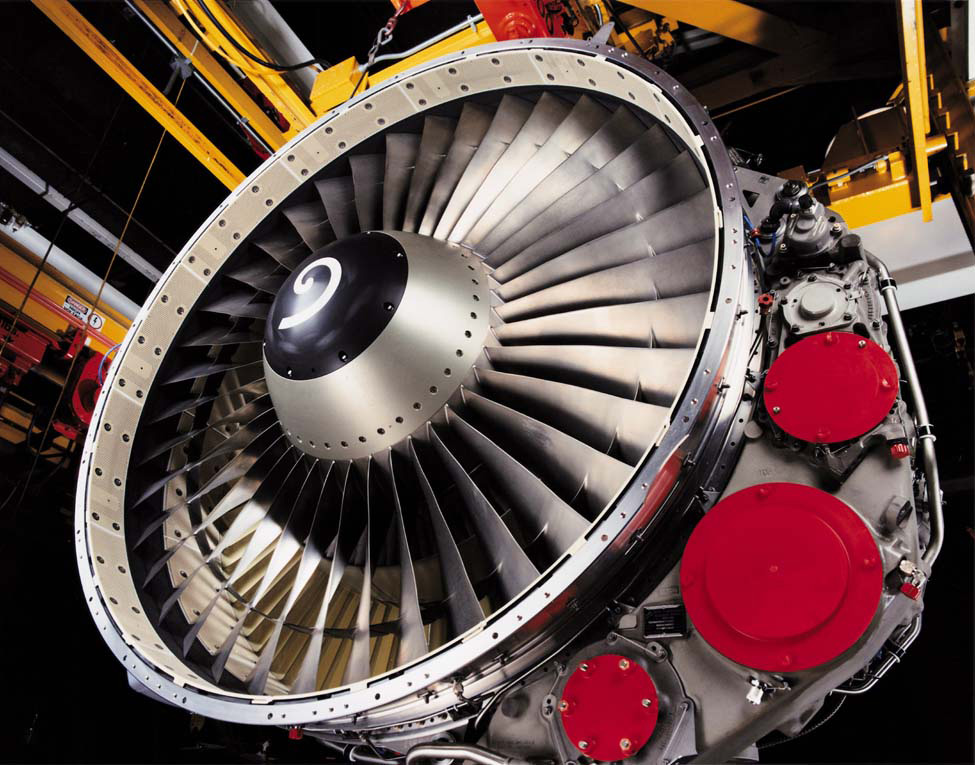
\includegraphics[scale=0.4]{CFM56-3C1-CFMi.jpg}
\captionof{figure}{Exemple d'un moteur à réaction en cours d'assemblage : le CFM56/General Electric F108}
\end{center}

De manière générale, ce relais d'accessoires se place dans la partie basse du moteur et aussi autour de la tuyère du réacteur.

\begin{center}
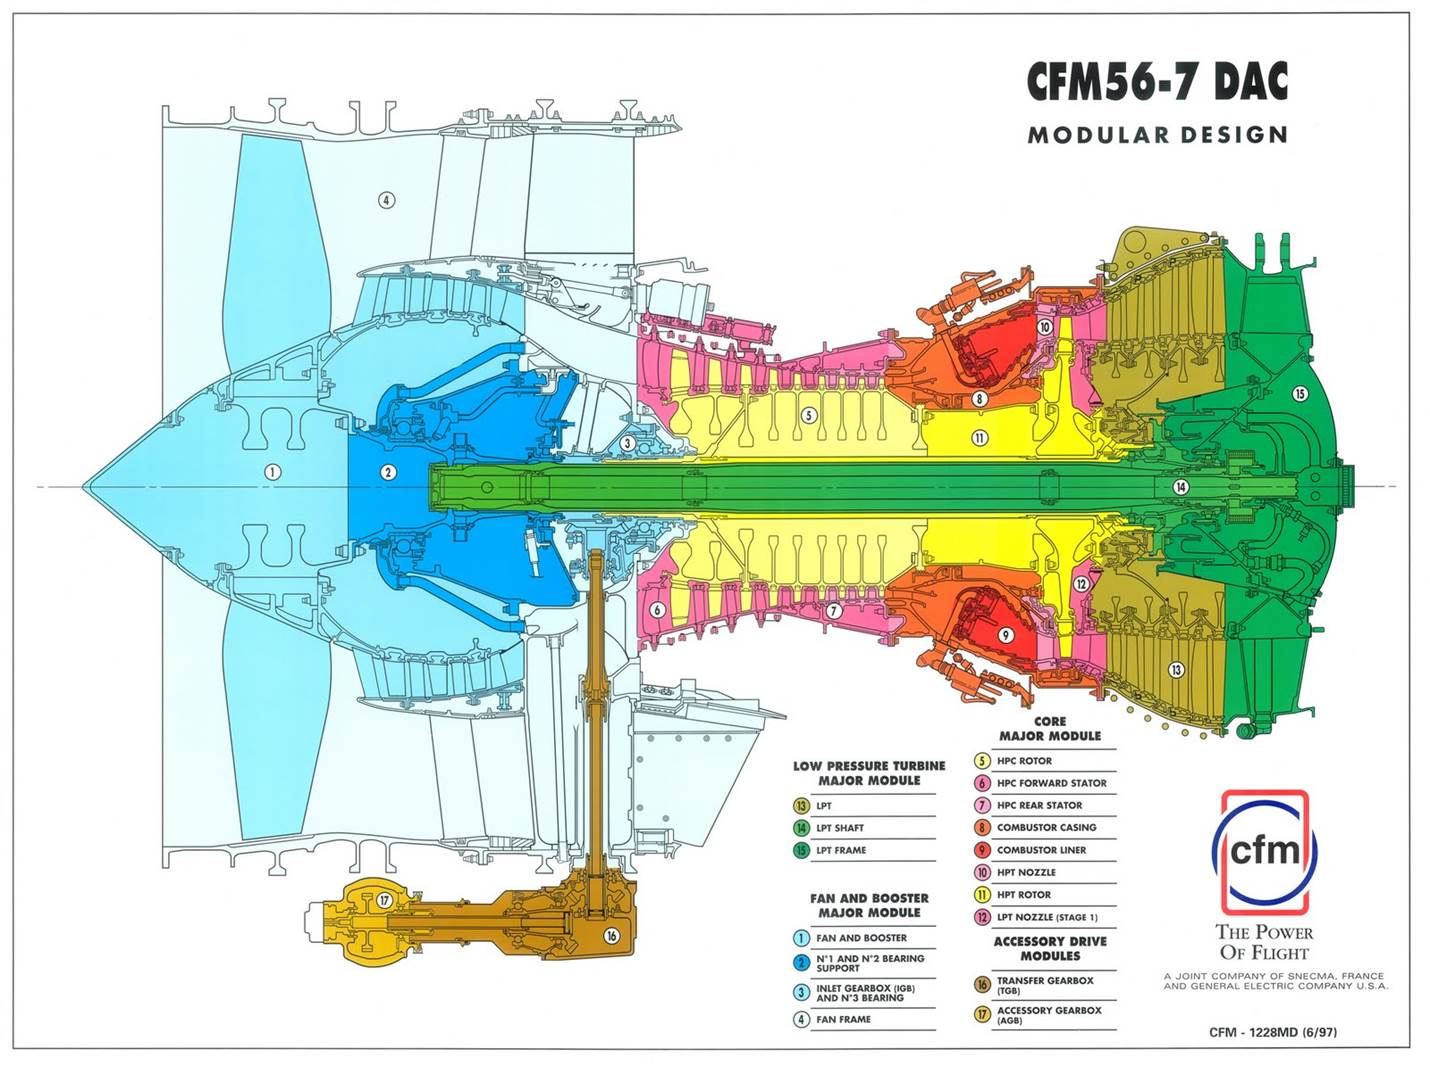
\includegraphics[scale=0.6]{CFM56-coupe.jpg}
\captionof{figure}{Vue de coupe du CFM56-7 DAC}
\end{center}

Comme nous pouvons le constater sur la vue en coupe du CFM56-7 DAC ci-dessus, le relais d'accessoires (qui est colorié en marron et possédant les numéros 16 et 17) est relié à l'arbre central du réacteur. Lors du démarrage du réacteur, le pilote de l'avion va demander le démarrage des différents composants sur le relais d'accessoires. Après avoir démarré ces derniers, l'arbre (numéro 16) va commencer à se mettre en rotation. Sa rotation va initialiser la rotation de l'arbre central ce qui va commencer à faire rentrer de l'air dans la tuyère. Une fois que le volume d'air dans la tuyère est suffisant, le carburant est injecté progressivement dans la zone à combustion pour permettre au réacteur jusqu'à atteindre un régime moteur suffisant pour l'auto-entretenir. Une fois que l'arbre central tourne suffisamment vite pour lui permettre de conserver son régime moteur en l'absence du relais d'accessoires, l'arbre venant du relais accessoires est débrayé.


\newpage
En regardant plus en profondeur un relais d'accessoires, nous remarquons la présence de nombreux composants et d'un jeu d'engrenage qui permet de faire la transmission de puissance entre les différents composants. La figure ci-dessous montre un relais d'accessoires de Rolls-Royce.
\begin{center}
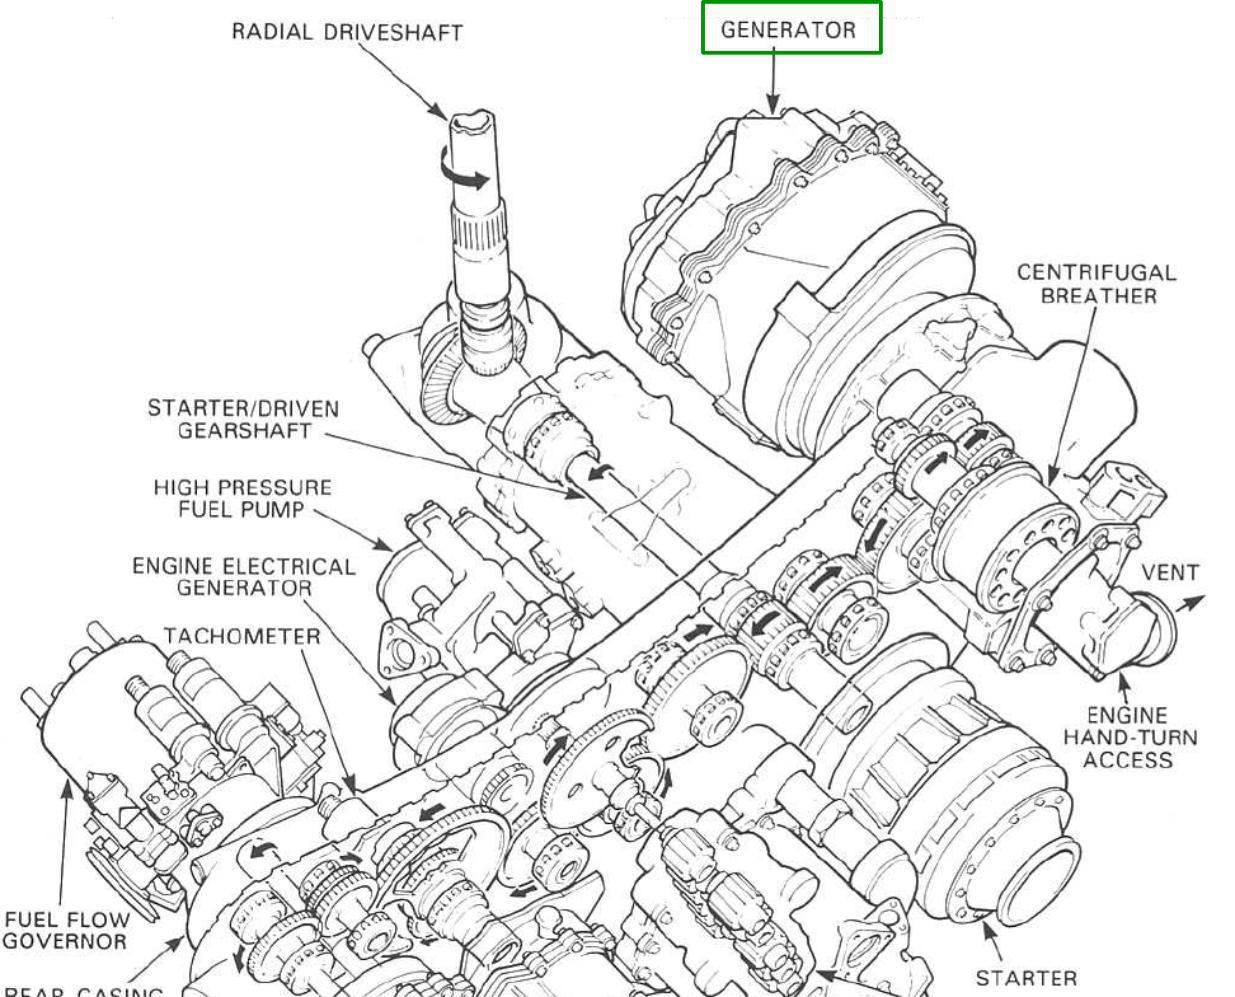
\includegraphics[scale=0.6]{relai_accessoires.jpg}
\captionof{figure}{Exemple d'un relais d'accessoires de Rolls-Royce}
\end{center}

Parmi les différents composants du relais d'accessoires, nous retrouvons une génératrice, un démarreur, des pompes hydrauliques et d'autres éléments indispensables pour le bon fonctionnement du réacteur d'avion. 
Il est important de signaler que les engrenages sont enfermés dans un carter et que ces engrenages sont imprégnés d'huile pour limiter les problèmes de contacts mécaniques. Une des pompe hydraulique est placé sur le relais d'accessoires pour permettre de maintenir un niveau d'huile suffisant dans le carter.

Dans le cadre de notre étude, nous allons concevoir un relais d'accessoires simplifié. En effet, nous avons à réaliser ce relais en plaçant un démarreur, une génératrice et deux pompes hydrauliques.


\newpage
\section{Recherche de la meilleure configuration}

Pour notre étude, nous avons cinq configurations possibles avec des architectures différentes. Nous avons deux architectures possibles autour du jeu d'engrenages. pour nos différents composants. La première configuration vise à placer notre quatre composants du même côté alors que la deuxième configuration vise à placer deux composants de chaque côté.
La figure ci-dessous montre les deux architectures possibles. "P1" et "P2" représentent les pompes hydrauliques, "G" la génératrice et "D" le démarreur. 

\begin{center}
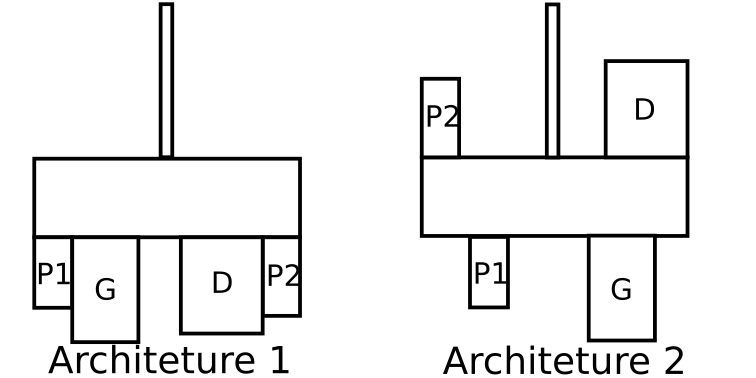
\includegraphics[scale=0.8]{architecture.png}
\captionof{figure}{Les deux architectures possibles pour notre relais d'accessoires}
\end{center}

Au total, nous avons dix combinaisons possibles avec les différents configurations et architectures possibles. Vous trouverez ci-dessous le tableau récapitulatif. Pour chaque choix de configuration, nous devrons utiliser des composants spécifiques.

% Please add the following required packages to your document preamble:
% \usepackage{graphicx}
\begin{table}[h]
\centering
\resizebox{\textwidth}{!}{%
\begin{tabular}{|l|l|l|l|l|l|}
\hline
Configurations & Architecture & Démarreur & Générateur & Pompe 1 & Pompe 2 \\ \hline
A1/A2 & 1 ou 2 & D1 & G1 & P4 & P5 \\ \hline
B1/B2 & 1 ou 2 & D2 & G2 & P1 & P4 \\ \hline
C1/C2 & 1 ou 2 & D3 & G3 & P2 & P4 \\ \hline
D1/D2 & 1 ou 2 & D4 & G4 & P3 & P4 \\ \hline
E1/E2 & 1 ou 2 & D5 & G5 & P2 & P3 \\ \hline
\end{tabular}%
}
\end{table}

Afin de choisir la meilleure configuration, nous avons réalisé deux études. La première est une étude de l'encombrement de l'ensemble des composants pour chaque configuration. La deuxième est  l'étude des rapports de réduction entre chaque composant pour chaque configuration.

\newpage
\subsection{Étude avec l'encombrement des différents composants}
Dans le but d'avoir un premier classement des différentes configurations en fonction de l'encombrement, nous avons étudié l'encombrement provoqué par chaque composant en variant les architectures possibles. 


Configuration A2 : Best
\newpage
\subsection{Étude avec les rapports de réduction}

Après avoir obtenu un premier classement pour les différentes configurations, nous avons étudié les rapports de réduction entre chaque composants pour chaque configuration possible. Au total, nous avons pu tester 480 combinaisons possibles ((1 (architecture 1) + 3 (architecture 2))$\times$ 4!$\times$ 5 (configurations) = 4$\times$24$\times$5 = 480). L'architecture 2 permet trois dispositions différentes car nous pouvons avoir le cas où les arbres de deux composants peuvent se connecter sur un arbre intermédiaire.

Pour effectuer un classement pertinent, nous avons décidé de classer les configurations en fonction de l'écart-type du cumul des rapports de réduction, du nombre d'engrenages ayant un rapport à l'extérieur de l'intervalle $[0,5,2]$ et du respect du sens de rotation du démarreur à air. En effet, en fonction de la configuration, le démarreur tourne dans le sens horaire ou dans le sens trigonométrique.

Vous pourrez trouver ci-dessous un exemple d'un tableau analysant les différentes combinaisons possibles pour la configuration A1.

% Please add the following required packages to your document preamble:
% \usepackage{graphicx}
\begin{table}[h]
\centering
\resizebox{\textwidth}{!}{%
\begin{tabular}{|l|l|l|l|l|l|}
\hline
Configuration & Entre 1 et 2 & Entre 2 et centre & Entre 3 et centre & Entre 4 et 3 & Écart-type \\ \hline
D1/G1/P4/P5 & 0,584 & 2,094 & 0,409 & 0,760 & 0,768513463 \\ \hline
D1/G1/P5/P4 & 0,584 & 2,094 & 0,311 & 1,316 & 0,80050416 \\ \hline
D1/P4/G1/P5 & 2,985 & 0,409 & 2,094 & 0,149 & 1,359131176 \\ \hline
D1/P5/G1/P4 & 3,929 & 0,311 & 2,094 & 0,195 & 1,760340963 \\ \hline
D1/P4/P5/G1 & 2,985 & 0,409 & 0,311 & 6,732 & 3,014414058 \\ \hline
D1/P5/P4/G1 & 3,929 & 0,311 & 0,409 & 5,115 & 2,45143273 \\ \hline
G1/D1/P4/P5 & 1,714 & 1,222 & 0,409 & 0,760 & 0,566371493 \\ \hline
G1/D1/P5/P4 & 1,714 & 1,222 & 0,311 & 1,316 & 0,592698574 \\ \hline
G1/P4/D1/P5 & 5,115 & 0,409 & 1,222 & 0,255 & 2,28308889 \\ \hline
G1/P5/D1/P4 & 6,732 & 0,311 & 1,222 & 0,335 & 3,083966172 \\ \hline
G1/P4/P5/D1 & 5,115 & 0,409 & 0,311 & 3,929 & 2,45143273 \\ \hline
G1/P5/P4/D1 & 6,732 & 0,311 & 0,409 & 2,985 & 3,014414058 \\ \hline
P4/G1/D1/P5 & 0,195 & 2,094 & 1,222 & 0,255 & 0,901206993 \\ \hline
P4/G1/P5/D1 & 0,195 & 2,094 & 0,311 & 3,929 & 1,760340963 \\ \hline
P4/D1/P5/G1 & 0,335 & 1,222 & 0,311 & 6,732 & 3,083966172 \\ \hline
P4/D1/G1/P5 & 0,335 & 1,222 & 2,094 & 0,255 & 0,864661744 \\ \hline
P4/P5/D1/G1 & 1,316 & 0,311 & 1,222 & 1,714 & 0,592698574 \\ \hline
P4/P5/G1/D1 & 1,316 & 0,311 & 2,094 & 0,584 & 0,80050416 \\ \hline
P5/D1/G1/P4 & 0,255 & 1,222 & 2,094 & 0,195 & 0,901206993 \\ \hline
P5/P4/G1/D1 & 0,760 & 0,409 & 2,094 & 0,584 & 0,768513463 \\ \hline
P5/P4/D1/G1 & 0,760 & 0,409 & 1,222 & 1,714 & 0,566371493 \\ \hline
P5/G1/P4/D1 & 0,149 & 2,094 & 0,409 & 2,985 & 1,359131176 \\ \hline
P5/D1/P4/G1 & 0,255 & 1,222 & 0,409 & 5,115 & 2,28308889 \\ \hline
P5/G1/D1/P4 & 0,149 & 2,094 & 1,222 & 0,335 & 0,895250311 \\ \hline
\end{tabular}%
}
\end{table}

Après avoir testé l'ensemble des combinaisons possibles pour une configuration, nous affichons les valeurs dans un graphique. Cela nous d'avoir plus rapidement la configuration la plus intéressante.

\begin{center}
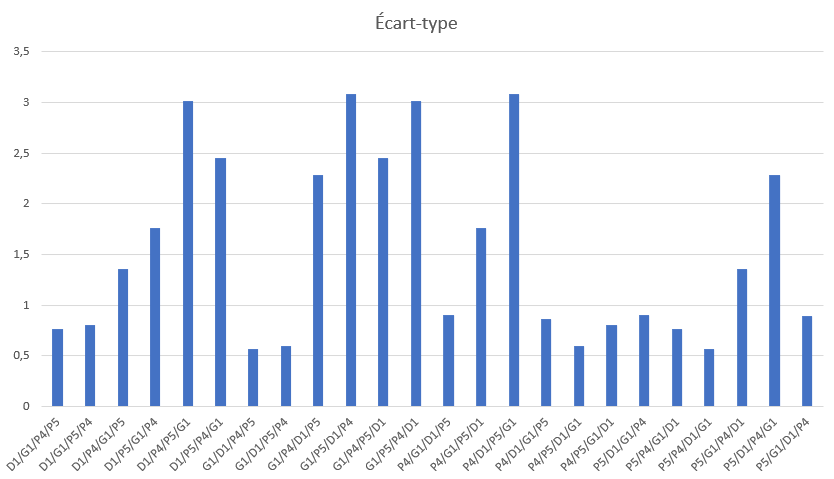
\includegraphics[scale=0.8]{graphique_ecart_type.PNG}
\captionof{figure}{Courbe récapitulant l'écart type pour la configuration A1}
\end{center}

Pour chaque configuration, nous avons testé l'ensemble des combinaisons possibles. Après avoir fait cela, nous avons affiché l'écart-type pour les quatre architectures possibles pour la configuration. La figure ci-dessous montre l'écart-type des différentes combinaisons possibles avec la configuration A.

\begin{center}
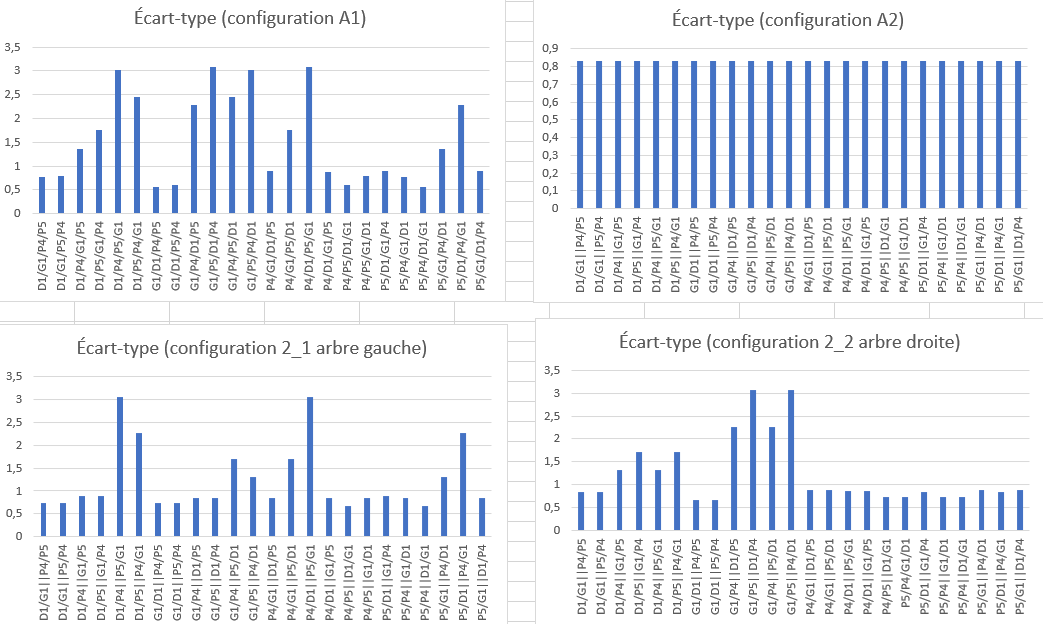
\includegraphics[scale=0.75]{graphique_ecart_type_configurationA.PNG}
\captionof{figure}{Courbes de l'écart-type des différentes combinaisons possibles avec la configuration A}
\end{center}

Après avoir testé les différents combinaisons, nous avons retenu les configurations suivantes : G1/D1/P4/P5 et G1/D1/P5/P4.

\begin{center}
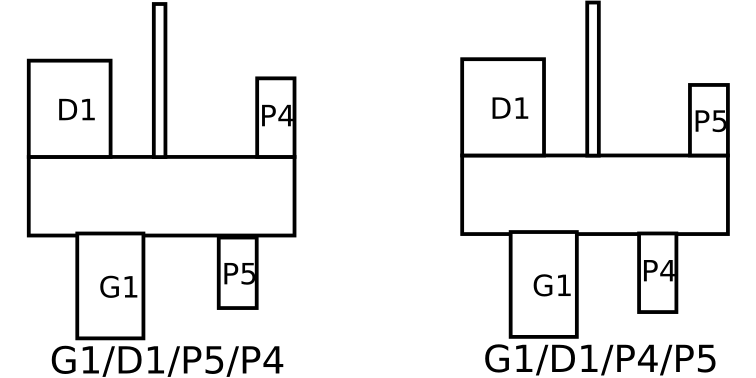
\includegraphics[scale=0.75]{conf_retenu.png}
\captionof{figure}{Les configurations retenues par notre équipe}
\end{center}

Le choix entre ces deux configurations va être fait en fonction de l'encombrement provoqué par le jeu d'engrenage pour chacune des configurations.

\newpage
\subsection{Choix de la meilleure configuration}
Schéma avec P5 en bas et P4 en haut

\section{Dimensionnement de notre relais d'accessoires}

\section{Conception sur Catia}
TestJerome


\end{spacing}
\end{document}

